% 设置页码计数器为 1 (也就是当前页面为第一页)
\setcounter{page}{1}

% ==================================================
% @brief    问题重述
% --------------------------------------------------

\mcmSection{问题重述}

\mcmSubsection{问题背景}

多波束测线技术是用来测量水体深度的技术。利用该技术,可以绘制出海床的地形图。规划航行路线,可以绘制出一定区间内的区域。但是海床的地形差异变化巨大,深浅不一会导致测绘系统的覆盖区域发生改变。如果测线过于密集,那么就会导致数据量过大,地形图绘制效率低下;如果过于稀疏,那么数据量过少,海床的某些区域没有探测到,地形图的绘制就会存在缺损。为了解决该问题,需要建立相关数学模型,规划测线路径,提高效率的同时,保证地形图绘制的准确性。

\mcmSubsection{具体问题重述}

\textbf{问题1:}根据题意,抽象出

\textbf{问题2:}

\textbf{问题3:}

\textbf{问题4:}

% ==================================================
% @brief    问题分析
% ==================================================

\mcmSection{问题分析}

\mcmSubsection{通过三角函数关系求出覆盖宽度}


% ==================================================
% @brief    模型假设
% ==================================================

\mcmSection{模型假设}

\begin{enumerate}
    \item 假设一
    \item 假设二
    \item 假设三
\end{enumerate}

% ==================================================
% @brief    模型假设$$
% ==================================================

\mcmSection{符号说明及名称定义}

\mcmSubsection{名称定义}

\begin{enumerate}
    \item \textbf{测垂面}是指与测线方向垂直的平面(如图\ref{fig:符号说明}中平面$GIH$);
    \item \textbf{测坡线}是指测线的测垂面与海底坡面的交线(如图\ref{fig:符号说明}中线段$IH$);
    \item \textbf{测坡角}是指测坡线与水平面的夹角(如图\ref{fig:符号说明}中线段$IH$与水平面的夹角);
    \item \textbf{海底坡面的倾斜角}是指海底坡面与水平面的夹角(如图\ref{fig:符号说明}中$\alpha$角)。\newline
\end{enumerate}

\begin{figure}[h]
    \centering
    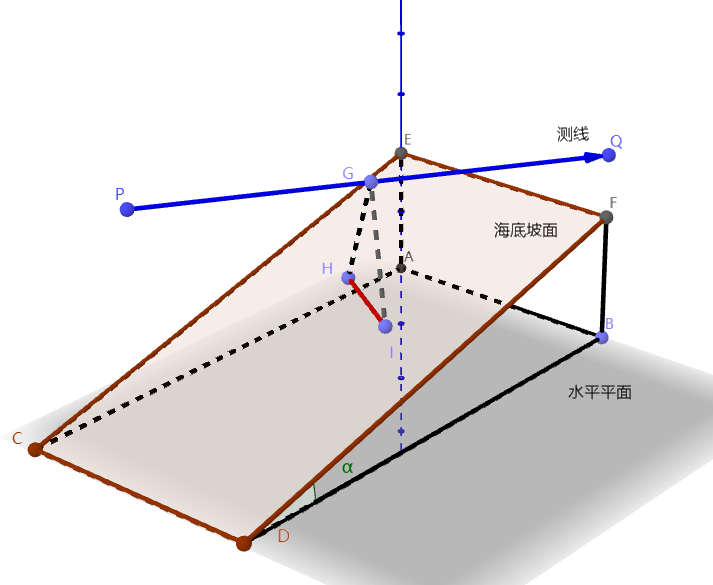
\includegraphics[scale=0.4]{res/img/符号说明.png}
    \caption{符号说明}
    \label{fig:符号说明}
\end{figure}


\mcmSubsection{符号说明}

\begin{table}[h]
    % 表格居中
    \centering

    % 调整行距
    \renewcommand\arraystretch{1.5}
    
    % 放缩表格
    \scalebox{1.2}{

        \begin{tabular}{cc}
        \hline
        \textbf{\fontsize{13}{1.5}{符号}}            & \textbf{\fontsize{13}{1.5}{意义}}                       \\ \hline

        $\alpha$     & 海底坡面的倾斜角     \\
        $\beta$      & 测线的方向角 \\
        $\gamma$       & 测坡角 \\ \hline
        \end{tabular}
    
    }
\end{table}
